\section{Background and System Description}\label{sec:hierarchical:related_work}

In this section we describe content popularity and traffic models used to evaluate the performance of contents delivery networks.
We describe the systems model for hierarchical caching systems.
We present a representative set of cache eviction policies and provide an overview of recent efforts in modeling the performance of isolated and interconnected caches.

\subsection{System Model for Hierarchical Caching Systems}\label{sec:hierarchical:system_model}

\begin{figure}[tb]
\centering
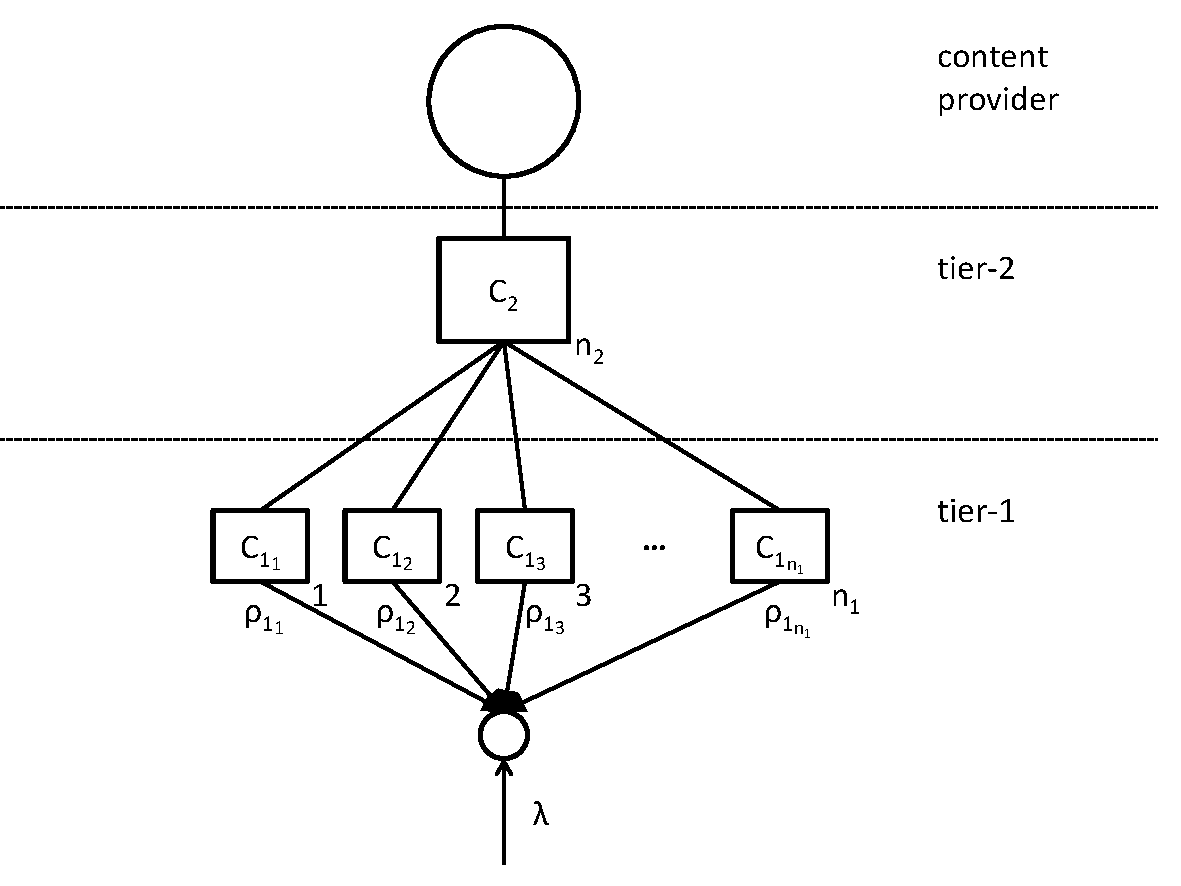
\includegraphics[width=75mm]{hierarchical/analyticbw/figures/hcmodeln1}
\caption{System model.}
\label{fig:hcmodel}
\end{figure}

To model the content delivery network, we consider a set of caches $\Gamma$ that is organized in a tiered caching architecture as depicted in figure~\ref{fig:hcmodel}. Each cache in $\Gamma$ has a certain cache capacity $C$, which specifies the number of content items it can store.
%TODO rephrase
%bin-packing problems can arise and therefore size has been considered as an important factor in studies which assume complete files as transport unit.
However, content delivery networks and peer-to-peer systems and coding schemes for video streams are segmenting data into small chunks in the kB range.
Therefore, we simply assume objects of fixed size corresponding to data chunks.
Consider that the method can also be applied to content with varying file size, if the sums are weighted accordingly.
Tier-1 caches have capacity $C_{1_i}, i\in\{1,...,n_1\}$ and tier-2 caches have capacity $C_{2_i}, i\in\{1,...,n_2\}$.
%We use the convention $C_1=C_{1_i}, \forall i$ if we assume the same cache size for all tier-1 caches.
Here we assume, that the cache capacity of all tier-1 caches is equal and use the convention $C_1=C_{1_i}, \forall i$.
This is for example the case if the caches are deployed by a provider on customer premise equipment.
If the caches are set up by end-users the cache capacities may vary.
Each tier-1 cache $i$ has a specific average upload throughput $\rho_{1_i}$.
Content items are requested from a catalog with size $N$.
Each item $m\in \{1,2,\dots,N\}$ is requested with rate $\lambda_m$.
The total arrival rate of requests is $\lambda=\sum_{m=1}^N \lambda_m$.
%\begin{equation}
%\lambda=\sum_{m=1}^N \lambda_m \, .
%\end{equation}

The arrival rate of requests for an item can then also be expressed with the probability $p_m$ that item $m$ is requested:

\begin{equation}
\lambda_m = p_m \lambda \, , \text{where} \, \sum_{m=1}^N p_m = 1 \, .
\end{equation}

%We consider a sharing probabilty $p_{share}$ which specifies the share of home routers in the AS that supports the caching functionality and serves as tier-1 cache.

%\begin{itemize}
%	\item Number IP-Adresses -> Number of Routers
%	\item Caches and Sharing Probability
%  	\item Replication Factor -> optimize with http://conferences.sigcomm.org/co-next/2009/papers/Valancius.pdf and http://arxiv.org/pdf/1004.4709.pdf
%  	\item Capacity of an AS, effective cache capacity
%    \item ratio upload download bandwidth -> should ISPs change their contracts?
%  \item locality of requests -> higher potential of the overlay
%\end{itemize}

\begin{table}[tb]
\centering
\caption{Notation of the paper.}
\label{tab:notation}
\begin{tabular}{|c|c|c|}
\hline
param. & description & default \\
\hline
$N$ & catalogue size & 1e6 \\
$n_{1}$ & number of tier-1 caches & 1e4 \\
$n_{2}$ & number of tier-2 caches & 1 \\
$C_{1}$ & tier-1 cache capacity & 8 \\
$C_{2}$ & tier-2 cache capacity & 1e4 \\
$\rho_{1}$ & tier-1 cache upload bandwidth & 0.8Mbps \\
$\lambda_m$ & arrival rate of requests for object $m$& \\
$b_m$ & bit rate of object $m$& \\
$d_m$ & duration of object $m$& \\
%%$\bar{\lambda}$ & average arrival rate of requests& \\
%$r_m$ & number of replications of object m& \\
\hline
\end{tabular}
\end{table}

\subsection{Content Popularity and Traffic Model}
The standard approach to characterize the pattern of object requests arriving at a cache is the Independent Reference Model (IRM) \cite{coffman1973operating}.
The IRM makes the following assumptions.

\newtheorem{irma}{Assumption}\begin{irma}\label{catalouge}
Users request objects from a catalogue with fixed size $N$.
\end{irma}
\newtheorem{irmb}[irma]{Assumption}\begin{irmb}\label{pmc}
The object popularity does not vary over time, i.e., the probability $p_m$ that an item $m, 1\leq m \leq N$ is requested, is constant.
\end{irmb}
\newtheorem{irmc}[irma]{Assumption}\begin{irmc}\label{iid}
The probability $p_m$ that an item is requested, is independent of all past requests, generating an i.i.d request process.
\end{irmc}

The IRM ignores temporal correlations in the request process.
In practice the popularity of content changes over time, such that the request rate increases if an object grows in popularity and decreases when the demand of the item drops. This effect is referred to as \textit{temporal locality}, i.e., when the request rate of an object increases in a short period of time.
This effect can have a strong positive impact on the efficiency of caching.

To account for temporal locality the request process can be modeled as renewal process \cite{martina2014unified} or as Markov modulated Poisson Process \cite{garetto2014dynamic}.
In these case the request process for each content is stationary.

In the renewal traffic model the request process for every content $m$ is described by an independent process with assigned inter-request time distribution.
The Markov modulated Poisson process models describes an ON-OFF process for a given content $m$.
The ON and OFF periods are exponentially distributed.
During an ON period the request rate for an item $\lambda_m$ is constant.
The model allows simple analysis if the OFF period is set much larger than the cache eviction time.
This makes the makes the probability negligible that an item $m$ is still in the cache at the end of its OFF period.

alternative SNM \cite{traverso2013temporal}
represent the overall request process as the superposition of a potentially infinite population of independent inhomogeneous Poisson processes (shots)

an ON
period  plays  exactly  the  same  role  as  a  (rectangular) shot  in
the SNM proposed in

however, the definition of analytical models for the evaluation of cache performance under the SNM
under the SNM traffic model can predicted with high accuracy by adopting a fixed-size content catalogue, and modeling the arrival process of each content by a renewal process with a specific inter-request time distribution

Zipf-Law

\subsection{Caching Strategies}

In the following we give a representative set of caching strategies.
The caching strategy decides which object in the cache is evicted if a newly requested item has to be stored in the cache.

\begin{itemize}
  \itemsep0em
  \item RANDOM: The simplest way to choose an item to make room for a new object is by random.
  \item LFU: The Least Frequently Used policy evicts the least frequently used item.
  It stores the most popular items in the cache.
  LFU performs optimal under IRM traffic.
  \item LRU: If a newly requested item is not in the cache, it is stored in the cache. The Least Recently Used item is evicted if the cache is full.
  A well known problem of LRU caches is cache pollution, which occurs if objects are replaced by less frequently requested items or items that are requested only once.
  \item q-LRU: If a newly requested item is not in the cache, it is stored in the cache with probability $q$. The Least Recently Used item is evicted if the cache is full.
  The probability ob being stored in the caches is higher for frequently requested objects, which prevents cache pollution. \cite{martina2014unified}
  \item k-LRU: In the k-LRU policy $k-1$ virtual caches storing only object hashes precede the actual cache $k$. An object is only stored in cache $i$, if it is found its preceding cache $i-1$. The eviction policy of the caches is LRU.
  The virtual caches function as filters to prevent cache pollution. \cite{martina2014unified}
  \item SG-LRU: Score Gated LRU caching strategies attributes a store to each object. A newly requested object is only stored in the cache if it has a higher score that the bottom object. The score functions can be based on statistics of past requests approaching the LFU policy if the memory is large. \cite{hasslinger2014caching}
  \item LRL: If the capacity of caches is limited to serve requests due to bandwidth or processing constraints, requests for an item are blocked although the item is stored in the cache. The Least Recently Lost strategy evicts the object for which a request was least recently or never blocked. \cite{leconte2014adaptive}
  %\item LBW: \cite{zhou2015unifying}
\end{itemize}

In a system of interconnected caches, such as the hierarchical caching system described in \refsec{sec:hierarchical:system_model}, requests that are cannot be served at one cache or in one tier produce a miss and are forwarded to the next tier.
In this way the requests traverse a route towards the repository which stores all objects, until they finally hit the target.
The following replication strategies for cache networks decide how the object is replicated on the route traversed by the request \cite{rossini2014coupling,martina2014unified}:

\begin{itemize}
  \item LCE (leave-copy-everywhere): the object is sent to all caches on the backward path.
  \item LCD (leave-copy-down): the object is sent only to the cache preceding the one in which the object is found.
  \item LCP (leave-copy-probabilistically): the object is sent with probability $q$ to each cache on the backward path.
\end{itemize}

\subsection{Performance Evaluation of Hierarchical Caching Systems}
The vast expansion of streaming services and content delivery networks (CDNs) suggests addressing content by content centric networking (CCN), to enable effective traffic management.
Addressing content instead of physical servers allows utilizing local resources.
To enable addressing, content is identified with unique names.
Available storage in routers is used to cache content in these approaches.
Since the tree like structure of the routers spreads on the way to the end user, the content replication scales with the content demand.
Simulative evaluation of tree like content delivery networks is provided in \cite{lareida2015augmenting} considering overlays and inter-domain traffic cost according to AS relationships.
In \cite{applegate2010optimal} hierarchical content delivery networks with bandwidth constraints are evaluated by simulation. The impact of using edge resources with limited capacity for content delivery on QoE is evaluated by means of simulation in \cite{info3-inproceedings-2015-530}.

\begin{sidewaystable}
  \centering
  \caption{Overview on literature on performance evaluation of caching systems TODO update policies / Methods / ....}
  \label{tab:litoverview}
  \resizebox{\textwidth}{!}{%
  \begin{tabular}{|l|p{1.5cm}|p{1.5cm}|p{1.5cm}|p{1.5cm}|p{1.5cm}|p{1.5cm}|} \hline
    \textbf{Study} & \textbf{Policies} & \textbf{Topology} & \textbf{Traffic Model} & \textbf{Constraints} & \textbf{Placement} & \textbf{Method} \\ \hline \hline
    Che et al. \cite{che2002hierarchical} & LRU & Hierarchical & Static - IRM & Cache capacity & No & Analysis \\ \hline
    Applegate et al. \cite{applegate2010optimal} & LRU & Hierarchical & Static - IRM & Cache capacity, bandwidth & No & Simulation \\ \hline
    Rosensweig et al. \cite{rosensweig2010approximate} & LRU & General cache networks & Static - IRM & Cache capacity & No & Analysis \\ \hline
    Fricker et al. \cite{fricker2012impact,fricker2012versatile} & LRU & Hierarchical & Static - IRM, Zipf, general & Cache capacity & No & Analysis \\ \hline
    Hasslinger et al. \cite{hasslinger2014caching} & LRU, SG-LRU, SLWND & Single cache & Static - IRM, Zipf & Cache capacity & No & Analysis \\ \hline
    Martina et al. \cite{martina2014unified} & LRU, q-LRU, k-LRU & General cache networks & Static - IRM, renewal & Cache capacity & No & Analysis \\ \hline
    Valancius et al. \cite{valancius2009greening} & LRU, HWC & Hierarchical & Trace & Cache capacity, bandwidth & HWC & Trace driven simulation \\ \hline
    Tan et al. \cite{tan2013optimal} & LRU, HWC & Hierarchical & Static - Zipf & Cache capacity, bandwidth & HWC & Optimization \\ \hline
    Leconte et al. \cite{leconte2014adaptive} & LRL & Hierarchical & Dynamic - Zipf & Cache capacity, bandwidth & LRL & TODO \\ \hline
    Zhou et al. \cite{zhou2015unifying} & LBW & Hierarchical & Dynamic - Zipf & Cache capacity, bandwidth & LBW & TODO \\ \hline
    Garetto et al. \cite{garetto2014dynamic} & LRU & Hierarchical & Dynamic - OnOff & Cache capacity & No & Analysis \\ \hline
Traverso et al. \cite{traverso2013temporal} & LRU & Single Cache & Dynamic - SNM & Cache capacity & No & Analysis \\ \hline
    Leconte et al. \cite{leconte2016dynamic} & LRU & Hierarchical & Dynamic - SNM & Cache capacity & No & Analysis \\ \hline
  \end{tabular}}
\end{sidewaystable}

% \definecolor{myGray}{RGB}{221,223,255}
% \begin{minipage}{\textwidth}
%     \centering
%     \captionsetup{type=table}
% 	\begin{tabularx}{\textwidth}{X|cc|cc|cc|cc|ccc|cc|cccc|}
% 		& \rotatebox{90}{on-the-spot offloading} & \rotatebox{90}{delayed offloading} & \rotatebox{90}{constant density (metropolitan area)} & \rotatebox{90}{\textcolor{red}{\textbf{variable}} density (countryside)} & \rotatebox{90}{vehicles} & \rotatebox{90}{human walk} & \rotatebox{90}{real movement traces} & \rotatebox{90}{mobility models} & \rotatebox{90}{real AP traces} & \rotatebox{90}{AP models} &\rotatebox{90}{considered private APs}& \rotatebox{90}{realistic request workload} & \rotatebox{90}{synthetic request workload} & \rotatebox{90}{uses prediction} & \rotatebox{90}{opportunistic communication} & \rotatebox{90}{measures energy consumption} & \rotatebox{90}{provides incentive mechanism}\\
% 		\hline
% 		Lee et al. \cite{howMuchCanWifiDeliver} & $\bullet$ & $\bullet$ & $\bullet$ & -- & -- & $\bullet$ & $\bullet$ & -- & $\bullet$ & -- & $\bullet$ & $\bullet$ & $\bullet$ & -- & -- & -- & -- \\
% 		Balasubramanian et al. \cite{augmentingMobile3G} & -- & $\bullet$ & $\bullet$ & -- & $\bullet$ & -- & $\bullet$ & -- & $\bullet$ & -- & -- & $\bullet$ & $\bullet$ & $\bullet$ & -- & $\bullet$ & -- \\
% 		Mota et al. \cite{APAvailabilityParis} & $\bullet$ & -- & $\bullet$ & -- & $\bullet$ & -- & $\bullet$ & -- & $\bullet$ & -- & $\bullet$ & -- & $\bullet$ & -- & --& -- & -- \\
% 		Bulut et al. \cite{wifiHotspotPlacement2} & $\bullet$ & -- & $\bullet$ & -- & $\bullet$ & -- & $\bullet$ & -- & -- & $\bullet$ & -- & -- & $\bullet$ & -- & --& -- & -- \\
% 		Zhang et al. \cite{optimalHandingBackPoint} & -- & $\bullet$ & $\bullet$ & -- & $\bullet$ & -- & $\bullet$ & -- & -- & $\bullet$ & -- & -- & $\bullet$ & $\bullet$ & -- & -- & -- \\
% 		Wiethölter et al. \cite{ChooseTrafficStreamOffloading} & $\bullet$ & -- & -- & -- & -- & -- & -- & $\bullet$ & -- & $\bullet$ & -- & -- & $\bullet$ & -- & -- & -- & -- \\
% 		Mehmeti et al. \cite{OnTheSpotOffloadingQueuingModel} & $\bullet$ & -- & -- & -- & -- & -- & -- & $\bullet$ & -- & $\bullet$ & -- & -- & $\bullet$ & -- & -- & -- & -- \\
% 		Lee et al. \cite{offloadingWithUserMobilityHistory} & -- & $\bullet$ & -- & -- & -- & -- & -- & $\bullet$ & -- & $\bullet$ & -- & -- & $\bullet$ & $\bullet$ & -- & -- & -- \\
% 		Guo et al. \cite{optimalScanningPeriod} & $\bullet$ & -- & $\bullet$ & -- & $\bullet$ & -- & -- & $\bullet$ & -- & $\bullet$ & -- & -- & $\bullet$ & -- & -- & $\bullet$ & -- \\
% 		Yoon et al. \cite{keepSessionSeamless} & $\bullet$ & -- & -- & -- & -- & -- & -- & ($\bullet$) & -- & ($\bullet$) & -- & -- & $\bullet$ & -- & -- & $\bullet$ & -- \\
% 		Go et al. \cite{disruptionTolerantProtocol} & $\bullet$ & -- & ($\bullet$) & -- & ($\bullet$) & ($\bullet$) & -- & ($\bullet$) & -- & ($\bullet$) & -- & -- & $\bullet$ & -- & -- & $\bullet$ & -- \\
% 		Dimatteo et al. \cite{DTNWithPocketSwitched} & -- & $\bullet$ & $\bullet$ & -- & $\bullet$ & -- & $\bullet$ & -- & -- & $\bullet$ & -- & -- & ($\bullet$) & -- & $\bullet$ & -- & -- \\
% 		Han et al. \cite{opportunisticCaseStudy} & -- & $\bullet$ & $\bullet$ & -- & -- & $\bullet$ & $\bullet$ & $\bullet$ & -- & -- & -- & -- & $\bullet$ & -- & $\bullet$ & ($\bullet$) & ($\bullet$) \\
% 		Barbera et al. \cite{VIPDelegation} & -- & $\bullet$ & $\bullet$ & -- & $\bullet$ & $\bullet$ & $\bullet$ & $\bullet$ & -- & -- & -- & -- & -- & ($\bullet$) & $\bullet$ & -- & -- \\
% 		Han et al. \cite{greenContentBroker} & $\bullet$ & ($\bullet$) & -- & -- & -- & -- & -- & $\bullet$ & -- & $\bullet$ & -- & -- & $\bullet$ & -- & $\bullet$ & $\bullet$ & -- \\
% 		Efstathiou et al. \cite{AnreizsystemeWifiCities} & $\bullet$ & -- & $\bullet$ & -- & -- & $\bullet$ & -- & $\bullet$ & -- & $\bullet$ & $\bullet$ & -- & $\bullet$ & -- & -- & -- & $\bullet$ \\
% 		Gao et al. \cite{IncentiveMobileDataOffloading} & $\bullet$ & -- & -- & -- & -- & -- & -- & $\bullet$ & -- & $\bullet$ & -- & -- & $\bullet$ & -- & -- & -- & $\bullet$ \\
% 		Zhuo et al. \cite{AnIncentiveFrameworkfor3G} & -- & $\bullet$ & $\bullet$ & -- & -- & $\bullet$ & $\bullet$ & -- & -- & -- & -- & -- & $\bullet$ & $\bullet$ & $\bullet$ & -- & $\bullet$ \\
% 		Lee et al. \cite{economicsOfWiFiOffloading} & $\bullet$ & $\bullet$ & $\bullet$ & -- & -- & $\bullet$ & $\bullet$ & -- & $\bullet$ & -- & -- & $\bullet$ & -- & -- & -- & -- & $\bullet$ \\
% 		Asheralieva et al. \cite{fonPerformance} & -- & -- & -- & -- & -- & -- & -- & $\bullet$ & -- & $\bullet$ & $\bullet$ & -- & $\bullet$ & -- & -- & -- & ($\bullet$) \\
% 		Mazloumian et al. \cite{optimalPricingStrategy} & -- & -- & -- & -- & -- & -- & -- & $\bullet$ & -- & $\bullet$ & -- & -- & ($\bullet$) & -- & -- & -- & $\bullet$ \\
% 		Iosifidis et al. \cite{EnablingCrowdSourcedMobileInternetAccess} & $\bullet$ & -- & -- & -- & -- & -- & -- & $\bullet$ & -- & $\bullet$ & -- & -- & $\bullet$ & -- & $\bullet$ & $\bullet$ & $\bullet$ \\
% 		\rowcolor{myGray} Our approach with varying user den\-si\-ties & $\bullet$ & -- & $\bullet$ & \large\textcolor{red}{$\bullet$} & $\bullet$ & -- & $\bullet$ & $\bullet$ & $\bullet$ & $\bullet$ & \textcolor{red}{$\bullet$} & -- & $\bullet$ & -- & -- & -- & \textcolor{red}{$\bullet$} \\
% 		\hline
% 	\end{tabularx}
% 	\captionof{table}{Overview of related publications for offloading}
% 	\label{relatedWorkOverview}
% \end{minipage}

\subsubsection{Analytic Model for LRU Caches}

In the following we give a brief overview of analytic models for the evaluation of mechanisms in CDN and CCN architectures.
In \cite{fricker2012impact} a two tiered caching architecture is investigated, where the first tier consists of home routers in access networks.
The second tier consists of data centers in the core network.
Requests that cannot be served in the first tier are forwarded to the second tier.
The popularity of objects follows a power-law and is modeled by the Zipf-law, which is observed for different types of content distributed in the Internet, including video \cite{gill2007youtube,cha2009analyzing}.
As cache replacement strategy Least-Recently-Used is assumed.
To analyse the performance of LRU caches, models exist that assume negative exponentially distributed inter-arrival times of object requests at the cache \cite{che2002hierarchical}.
The requests are generated according to the independent reference model (IRM), which assumes identically and independently distributed requests of a set of objects.
It is shown in \cite{fricker2012versatile} that the model also applies in more general conditions.
The model also provides accurate results for a high number of objects with varying file sizes.
In \cite{martina2014unified} the model is extended, to analyze advanced caching strategies like {$k$-LRU}, where objects have to pass a certain number of $k-1$ virtual caches to be stored in the actual cache.
The virtual caches replace objects according to LRU and store only meta information.
The IRM assumptions are generalized in order to apply to effects of temporal locality in the request process.
The model for LRU can be further extended to evaluate the performance of general cache networks \cite{rosensweig2010approximate, martina2014unified}.
Further caching strategies with limited memory, like W-LFU and Geometrical Fading, are investigated in \cite{hasslinger2014caching}.
The Sliding Window strategy applies the LFU approach to the frequency of requests in a limited time frame.
Geometrical Fading scores recent requests with a factor that decreases according to a geometric sequences with the number of intermediate request.

\subsubsection{Evaluation of Caching Systems with Limited Capacity}

The analytic models do not consider the service time of requests, which is limited by the bandwidth of the uplink of the cache.
In this work we consider a tiered caching architecture, where the upload bandwidth of the caches is highly limited.
%A limited bandwidth or service time of the caches is not considered in any of the above analytic models.
The paper closest to this works is \cite{valancius2009greening} which proposes the NaDa approach and develops an optimal content placement on NaDas.
The performance of the approach is evaluated with traces only.
To determine the performance analytically the system with bandwidth constraints is modeled as loss network consisting of a server for each of the caches. The exact stationary distribution of the loss network is too complex to evaluate.
In \cite{tan2013optimal} the system is analyzed under large system asymptotics where simplifications occur.
Wieso large system asymptotics ungeeignet

We use a different approach by approximating the arrival of rate requests.
This allows us to effectively assess the loss probability by using a simple form of the Erlang formula for a loss network.
%We combine the

To optimize the content placement adaptively \cite{leconte2014adaptive} propose Least-Recently-Lost (LRL) replacement, which tries to optimize the loss rate in the first tier.
A different approach is proposed by \cite{zhou2015unifying} which allocates bandwidth resources instead of content copies proportionally to the content popularity.

\subsubsection{Evaluation of Caching Systems with Dynamic Content Popularity}

renewal hyper-exponential \cite{martina2014unified}
exhibit dynamics in content popularity \cite{garetto2014dynamic} using an on-off-modulated process.
In \cite{leconte2016dynamic} the analysis is further extended for caches with small population, such as local caches considered in this study that are placed on home routers or set-top boxes.

\subsubsection{Content Placement}
hot warm cold
"Optimal content placement for a large-scale VoD system"
